\documentclass[a4paper,12pt]{article}

\usepackage{tocloft}
\usepackage{algorithmic}
\usepackage{algorithm}

\setlength{\cftbeforesecskip}{0.2cm}
% Enter the inputs below
%-------------------------------------------------------------------------------
\newcommand{\studentName}{David Korčák}
\newcommand{\projectTitle}{GPU-based simulation and reinforcement learning pipeline for tracked ground robots}
\newcommand{\academicYear}{Prague, January 2025}
\newcommand{\docType}{B4BPROJ6 report}
\newcommand{\studyProgramme}{Open Informatics}
\newcommand{\branchOfStudy}{Artificial Intelligence and Computer Science}
\newcommand{\supervisorName}{doc. Ing. Karel Zimmermann, Ph.D.}
%-------------------------------------------------------------------------------

% Style file (.sty) with dissertation format
\usepackage{report_template}


\begin{document}


% TITLE AND DECLARATION PAGESFluids_MSc_DissertationFluids_MSc_Dissertation
%------------------------------------------------------------------------
\frontMatter
%------------------------------------------------------------------------


% ABSTRACT
%------------------------------------------------------------------------
\section*{Abbreviations}
\label{sec:abbreviations}
\addcontentsline{toc}{section}{Abbreviations}

\textbf{MPC} - Model Predictive Control \\ 
\textbf{RL} - Reinforcement Learning \\
\textbf{MARV} - Mobile Advanced Robotic Vehicle \\
\textbf{TRADR} - Tracked Disaster Response Robot \\
\textbf{DoF} - Degrees of Freedom \\
\textbf{LiDAR} - Light Detection and Ranging \\
\textbf{CoG} - Center of Gravity \\
\textbf{GPU} - Graphics Processing Unit \\
\textbf{CPU} - Central Processing Unit \\
\textbf{RAM} - Random Access Memory \\
\textbf{VRAM} - Video Random Access Memory \\
\textbf{BVH} - Bounding Volume Hierarchy \\
\textbf{API} - Application Programming Interface \\
%------------------------------------------------------------------------

\clearpage
\pagestyle{fancy}


% TABLE OF CONTENTS
%------------------------------------------------------------------------
% \vspace*{-2cm} % adjust the spacing as needed
\tableofcontents % Use \thispagestyle for correct headers and footers
%------------------------------------------------------------------------


\clearpage

% INTRODUCTION
%------------------------------------------------------------------------
\section{Introduction}
\label{sec:introduction}

In many robotics applications, simulation is a key component of development, testing, and in some particular cases, the deployment. Control and planning algorithms benefit greatly from high simulation accuracy, however, the computational cost of such simulations can be prohibitive. Certain methods requiring high number of time steps or large sample sizes can become infeasible to run and quickly iterate over. 

Two such areas are Model Predictive Control (MPC) and Reinforcement Learning (RL). MPC performs optimization over a finite horizon, requiring multiple simulation rollouts to find the optimal control sequence. RL, on the other hand, requires a large number of samples to learn the optimal policy. Both of these methods are known for leading to state-of-the-art results. In particular, they can solve complex, high-DoF control problems with relatively little manual engieering or tuning, mostly through an appropriate penalty (reward) function. Therefore, it makes sense to investigate and optimize the simulation pipeline to make these methods more accessible and more widely applicable.

The aim of this project is to enable the use of these methods on tracked robots used by the Vision for Robotics and Autonomous Systems group by developing a GPU-based simulation pipeline, capable of running multiple times faster than real-time. The underlying simulation engine will be based on formulation proposed by \citet{Agishev_2024}. The engine will be integrated into a PyTorch-native \citep{paszke2019pytorchimperativestylehighperformance} simulation and reinforcement learning toolkit based on TorchRL \citep{bou2023torchrldatadrivendecisionmakinglibrary}. The pipeline will be evaluated on throughput (performance scaling with respect to the number of robots simulated at once) and the corresponding speedup over real time with respect to the length of integration step.





\clearpage


% BACKGROUND
%------------------------------------------------------------------------
\section{Background}
\label{sec:background}

Due to the popularity of Reinforcement Learning (RL) and Model Predictive Control (MPC) in robotics, there is a growing selection of simulation environments that are designed to be used with these methods. Honorable mentions include Farama's Gymnasium (continuation of the OpenAI gym) \citep{towers2024gymnasiumstandardinterfacereinforcement}, Google DeepMind's MuJoCo \citep{todorov2012mujoco} and DM Control suites, Google's BRAX \citep{brax2021github}, and the recently-released Genesis \citep{Genesis}.

While these engines are highly optimized, in some cases provide native interop with accelerator-friendly computation libraries such a JAX or PyTorch, and offer great flexibility for modeling of robots, none of them natively support robots with tracked (or wheeled) propulsion. They are designed for robotics with flexible joints and rigid bodies.

It is therefore necessary to develop a custom simulation engine capable of simulating tracked robots.
%------------------------------------------------------------------------


\clearpage


\section{Simulation of tracked robots}
\label{sec:robots_props}

\subsection{Tracked robots}
\label{sec:robots}

The Vision for Robotics and Autonomous Systems group utilises 2 kinds of tracked robots, each with a different propulsion setup. The first robot is \textbf{MARV} (Mobile Advanced Robotic Vehicle), developed by \href{https://jettyvision.cz/servisni-robot-marv/}{JettyVision}. It is a battery-powered robot with 4 independent tracks, each driven by a separate motor. Each of the tracks is capable of rotating around its main motor axis on a 180-degree arc, allowing the robot to conform to uneven terrain. In the rest of the report, these rotating tracks will be referred to as \textit{flippers}.

\begin{figure}[!h]
  \centering
  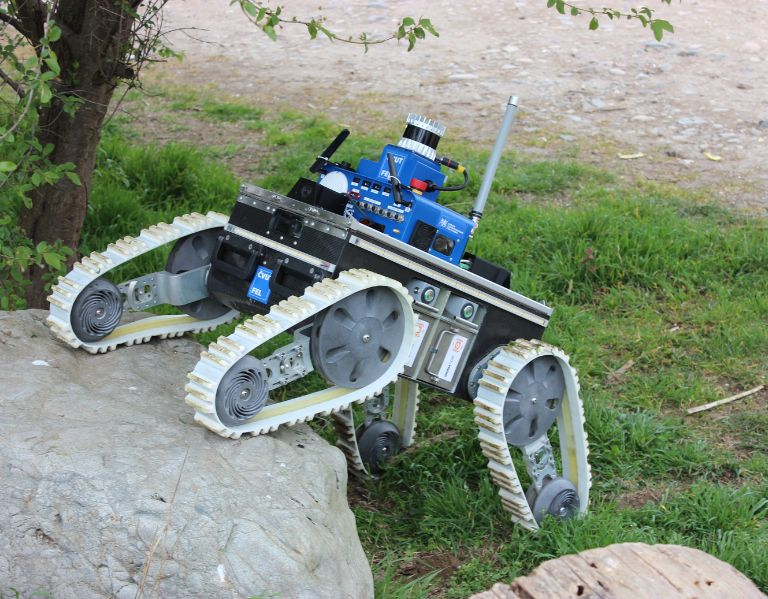
\includegraphics[width=0.4\textwidth]{fig/marv.jpg}
  \caption{MARV robot \citep{MARVphoto}}
  \label{fig:marv}
\end{figure}

The second robot, codenamed \textbf{TRADR}, was developed within the \href{https://www.tradr-project.eu/}{TRADR project}. Designed as a disaster-response robot, it is equipped with a more elaborate traction setup than \textit{MARV}. It features 4 flippers and adds a wide, fixed track along the robot's entire length on each side. The flippers share their rotation axes with the fixed track's wheels. 

\begin{figure}[!h]
  \centering
  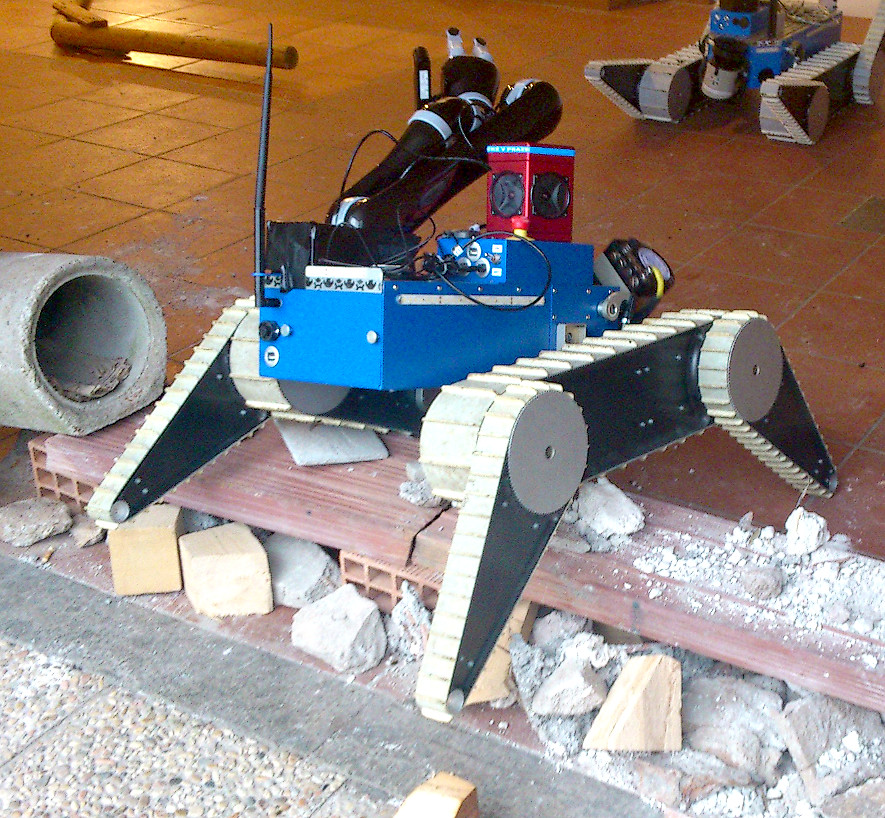
\includegraphics[width=0.4\textwidth]{fig/tradr.jpg}
  \caption{TRADR robot \citep{TRADRphoto}}
  \label{fig:tradr}
\end{figure}

Both robots can reach speeds of up to 1 m/s and are capable of off-road operation.

\clearpage

\subsection{Robot modeling}
\label{sec:modeling}
\subsubsection{Simplification of robot geometry}
For each of the robots, high-resolution triangular meshes are available. However, they are highly detailed and contain many unnecessary vertices, especially in details such as the cameras, LiDAR, or other small components. Because these parts of the robot never come into contact with the environment, they can be removed. Further details such as battery trays are not relevant either. This allows for a significant reduction in the number of vertices in the irrelevant parts of the robot. Overall, the most crucial component for collision detection and contact force computation is the flipper itself. Therefore, an elaborate process of simplifying the flippers' geometry and extracting their surface is used, while the rest of the robot is simplified by voxelization of a delaunay-triangulated envelope. The entire process of simplifying the robot geometry is shown in Algorithm~\ref{alg:mesh_simplification}.

\begin{algorithm}[H]
  \caption{Simplification of Robot Geometry  - see \href{https://github.com/edavidk7/tracked_sim_rl/blob/main/configs/robot_config.py\#L143}{code}}
  \label{alg:mesh_simplification}
  \begin{algorithmic}
    \vspace{0.25cm}
    \STATE \textbf{Procedure} ExtractSurfaceFromMesh(\textit{mesh}, \textit{n\_points}, \textit{clus\_opts})
        \STATE Perform Delaunay 3D triangulation on \textit{mesh}
        \STATE Extract the surface geometry
        \STATE Cluster surface points to \textit{n\_points}
        \RETURN Clustered centroids as \textit{Tensor}
    \vspace{0.25cm}

    \STATE \textbf{Procedure} SimplifyDrivingPart(\textit{mesh}, \textit{n\_points}, \textit{clus\_opts}, \textit{voxel\_size})
        \STATE Subsample points using ClusterPoints(\textit{mesh.points}, \textit{n\_points}, \textit{clus\_opts})
        \STATE Voxelize subsampled mesh using VoxelizeMesh(\textit{mesh}, \textit{voxel\_size})
        \RETURN Simplified mesh for driving part
        \vspace{0.25cm}
    \STATE \textbf{Procedure} SimplifyRobotBody(\textit{mesh}, \textit{n\_points}, \textit{clus\_opts}, \textit{voxel\_size})
        \STATE Extract \textit{surface} from \textit{mesh} using Delaunay3D
        \STATE Voxelize surface using VoxelizeMesh(\textit{surface}, \textit{voxel\_size})
        \RETURN Voxel centroids 
      \vspace{0.25cm}
    \STATE \textbf{Procedure} SimplifyRobotGeometry(\textit{body\_mesh}, \textit{part\_meshes}, \textit{n\_points}, \textit{clus\_opts}, \textit{voxel\_size})

      \STATE Simplify the body mesh using SimplifyRobotBody(\textit{body\_mesh}, \textit{n\_points}, \textit{clus\_opts}, \textit{voxel\_size})

        \FOR{\textbf{each} \textit{part\_mesh} in \textit{part\_meshes}}
            \STATE Simplify \textit{part\_mesh} using SimplifyDrivingPart(\textit{part\_mesh}, \textit{n\_points}, \textit{clus\_opts}, \textit{voxel\_size})
        \ENDFOR
        \RETURN Simplified robot geometry
        \vspace{0.25cm}
    \end{algorithmic}
    
  \end{algorithm}


\clearpage

\begin{figure}
  \centering
  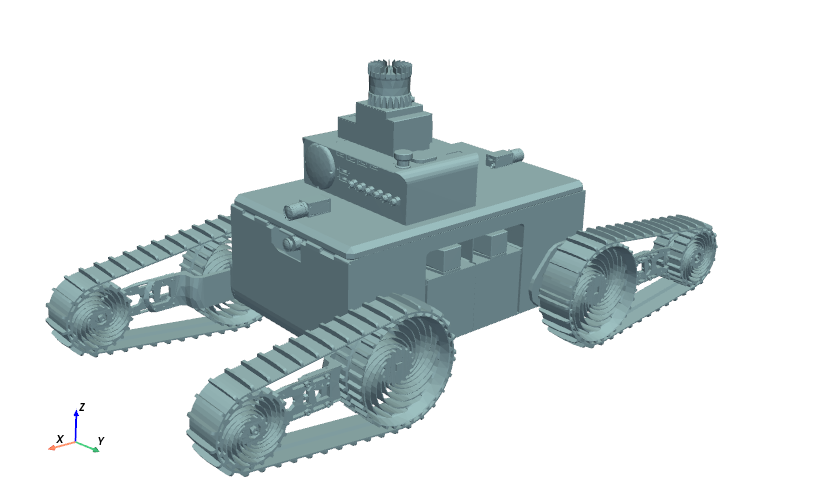
\includegraphics[width=0.6\textwidth]{fig/full_marv_mesh.png}
  \caption{Full MARV mesh}
  \label{fig:full_marv_mesh}
\end{figure}

\begin{figure}[H]
  \centering
  % row 1
  \begin{subfigure}[t]{0.45\textwidth}
      \centering
      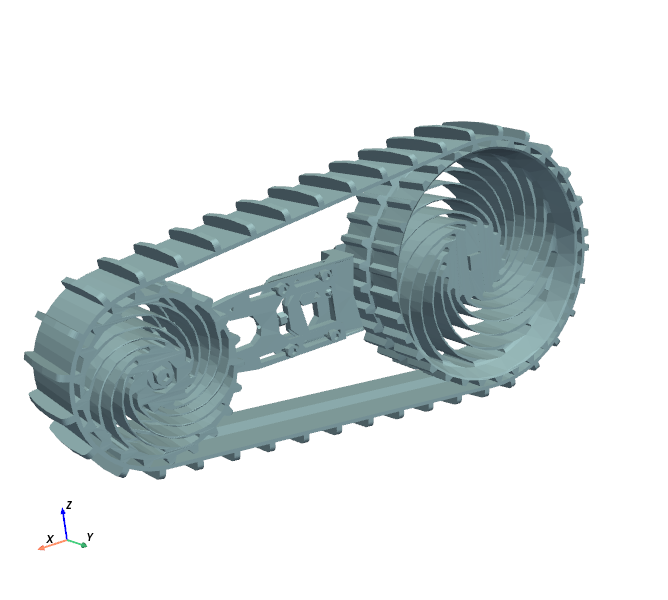
\includegraphics[width=\textwidth]{fig/full_flipper_mesh.png} % replace with your image path
      \caption{Full flipper mesh.}
      \label{fig:fig1}
  \end{subfigure}
  \hfill
  \begin{subfigure}[t]{0.45\textwidth}
      \centering
      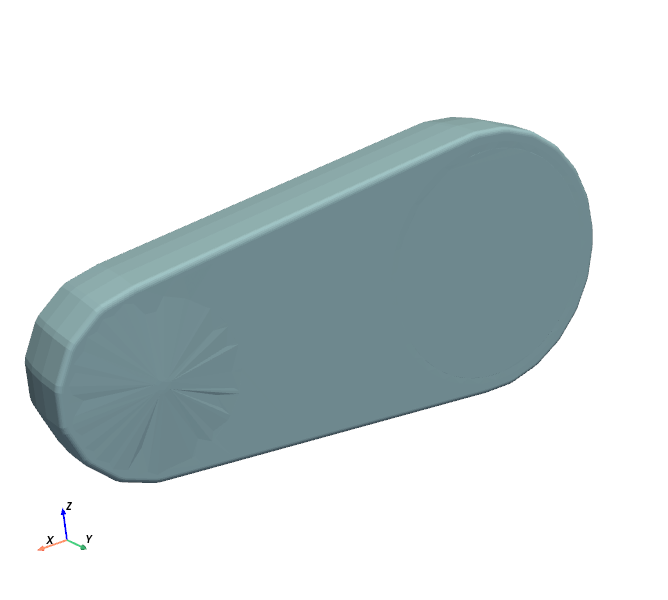
\includegraphics[width=\textwidth]{fig/flipper_delaunay.png} % replace with your image path
      \caption{3D Delaunay triangulation of the flipper mesh.}
      \label{fig:fig2}
  \end{subfigure}

  \vspace{0.5cm} % spacing between rows

  % row 2
  \begin{subfigure}[t]{0.45\textwidth}
      \centering
      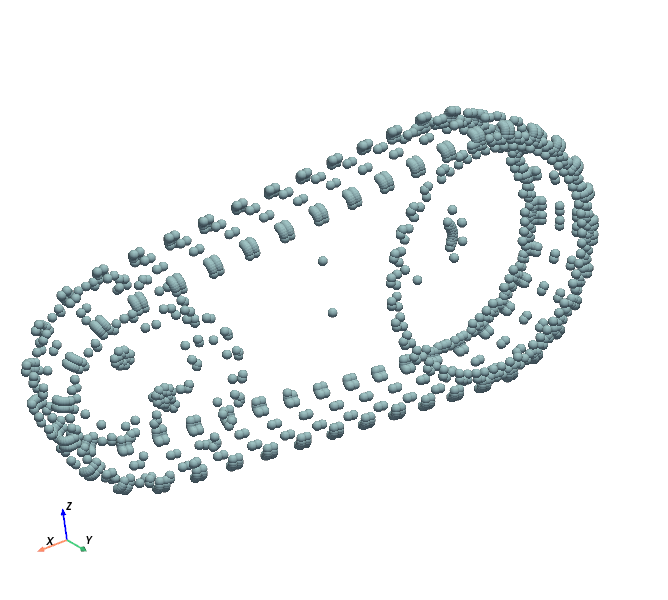
\includegraphics[width=\textwidth]{fig/flipper_surface_points.png} % replace with your image path
      \caption{Extracted surface points.}
      \label{fig:fig3}
  \end{subfigure}
  \hfill
  \begin{subfigure}[t]{0.45\textwidth}
      \centering
      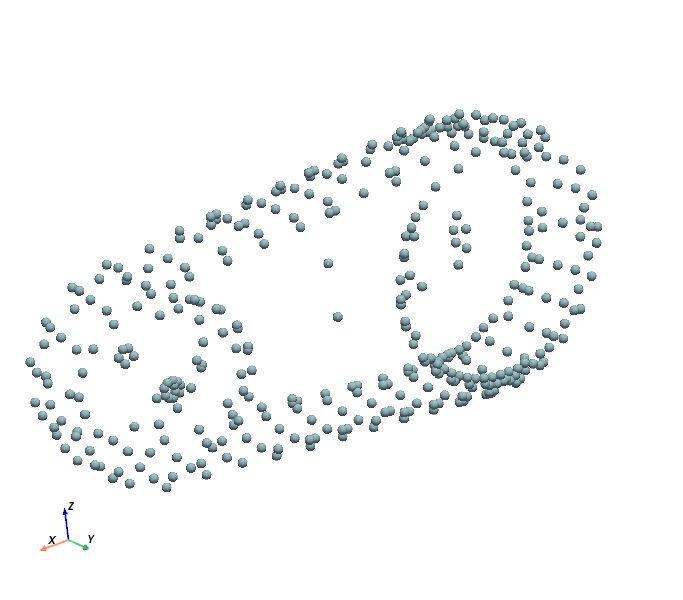
\includegraphics[width=\textwidth]{fig/flipper_clustered.png} % replace with your image paths
      \caption{Clustered surface points.}
      \label{fig:fig4}
  \end{subfigure}

  \caption{Simplification of the flipper geometry.}
  \label{fig:4figures}
\end{figure}

\clearpage

\subsubsection{Inertial properties} 
The robots' inertial properties are crucial for the simulation's accuracy, especially the force interactions. Here, we improve greatly over \citet{Agishev_2024}, where the robot's mass was distributed uniformly across the robot's points (globally simplified by voxelization). This is not realistic, as the robot's mass is concentrated in the robot's body (due to the presence of batteries, onboard computer, and sensors). Futher, the difference in point-per-unit-volume between the flippers and body parts of the mesh would lead to erroneous Center-of-Gravity placement and moment of inertia.

We address this with a simple modification. We model the discrepancy in volumetric density between the body and the flippers by assigning a lower relative mass to points in the flippers. The body's density is set to 1, while the flippers' density $\rho_\text{driving parts} \in \left(0.1,0.5\right)$. Using this modification, we distribute the mass of the robot in a pointwise fashion. Let $m$ be the total mass of the robot. Then, the mass of each point $i$ is given by Equation~\ref{eq:mass_distribution}, \href{https://github.com/edavidk7/tracked_sim_rl/blob/main/configs/robot_config.py\#L173}{code}.

\begin{equation}
  \label{eq:mass_distribution}
  m_i = \begin{cases}
    \frac{1}{Z} \cdot m & \text{if } i \in \text{body} \\
    \frac{\rho_\text{driving parts}}{Z} \cdot m & \text{if } i \in \text{driving parts}
  \end{cases} 
\end{equation}

where $Z = \sum_{i} \llbracket {i \in \text{body}} \rrbracket + \rho_\text{driving parts} \cdot \sum_{i} \llbracket {i \in \text{driving parts}} \rrbracket$ is the normalization constant. 

\subsubsection{Controls and kinematics}

To model the robot's propulsion, we relax the accuracy of the simulation and use a very simplified setup. The control velocity modeled by four scalar velocities, each corresponding to the speed of the track at the point of contact with the ground. Velocity vectors of each track are acting the robot's local x-coordinate, or its forward-facing direction (positive x). The robot's rotational velocity is generated by varying the speeds of the tracks between the left and right side. This is the simplest possible model of a tracked robot's kinematics, and it is part of our future work to improve it. As mentioned in Section \ref{sec:background}, none of the widely used simulation toolkits support tracked robots, as it is a very complex problem to solve, \href{https://github.com/edavidk7/tracked_sim_rl/blob/main/engine/engine.py#L147}{code}.

The control input for the flippers' articulation is a tuple of 4 scalar values, each representing the rotational velocity of the flipper around its y-axis, \href{https://github.com/edavidk7/tracked_sim_rl/blob/main/engine/engine.py#L92}{code}.

Overall, our control vector is $\mathbf{u} = \left(v_1, v_2, v_3, v_4, \omega_1, \omega_2, \omega_3, \omega_4\right)$, where $v_i$ is the velocity of the $i$-th track and $\omega_i$ is the rotational velocity of the $i$-th flipper.

\section{Physics simulation engine}
\label{sec:engine}

The key idea of the physics engine is to use a pointcloud representing the robot to perform all collision and environment interactions. This deviates from the standard practice of general engines computing collisions between triangular meshes with algorithms such as BVH. However, as described in Section \ref{sec:terrain}, it is sufficient to model the robot as a pointcloud in our case.



\subsection{Terrain modeling}
\label{sec:terrain}
We represent the terrain by an $N \times N$ grid $\mathbf{T}$ of metric height values. Formally, this corresponds to the discretization of some parameterized surface $\tau$ representing the real continuous terrain, into cells of size $d_c \times d_c$ where $d_c$ is a configurable metric value. The terrain grid is, of course, finite, with the origin $(0,0)$ located in the middle and the maximum absolute coordinate given by $d_{\text{max}}$. The grid size $N$ is given by $\lfloor {2\cdot \frac{d_{\text{max}}}{d_c}} \rfloor$.

\begin{figure}[H]
  \centering
  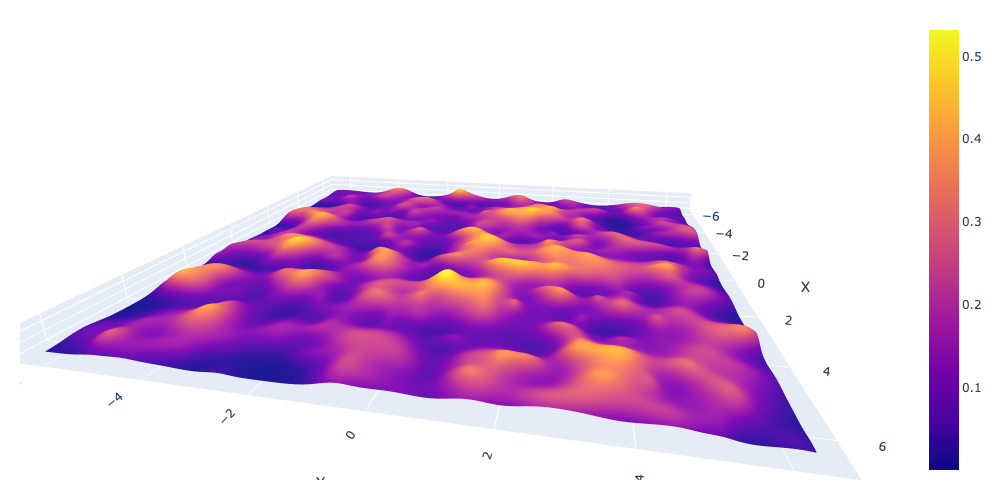
\includegraphics[width=0.8\textwidth]{fig/terrain.png}
  \caption{Example of 3D surface representing the terrain.}
  \label{fig:terrain}
\end{figure}

Then the cell at position $(i,j)$ in the grid represents the terrain height given as $\tau(i \cdot d_c + \frac{d_c}{2} - d_{\text{max}}, j \cdot d_c + \frac{d_c}{2} - d_{\text{max}}, \mathbf{T}\left[i,j\right])$. It is important to note that in this simulation, the terrain is the only other object in the world, and it is not moving. This allows us to greatly simplify the collision detection. We can detect whether the robot has penetrated the terrain simply by comparing the z-coordinate of its points with the height of the terrain at the same $x,y$ coordinates. The height of the terrain at those coordinates may be obtained by e.g. simple bilinear interpolation of the discrete grid. See \href{https://github.com/edavidk7/tracked_sim_rl/blob/main/configs/world_config.py}{code 1}, \href{https://github.com/edavidk7/tracked_sim_rl/blob/main/utils/environment.py}{code 2}. 

\begin{figure}[H]
  \centering
  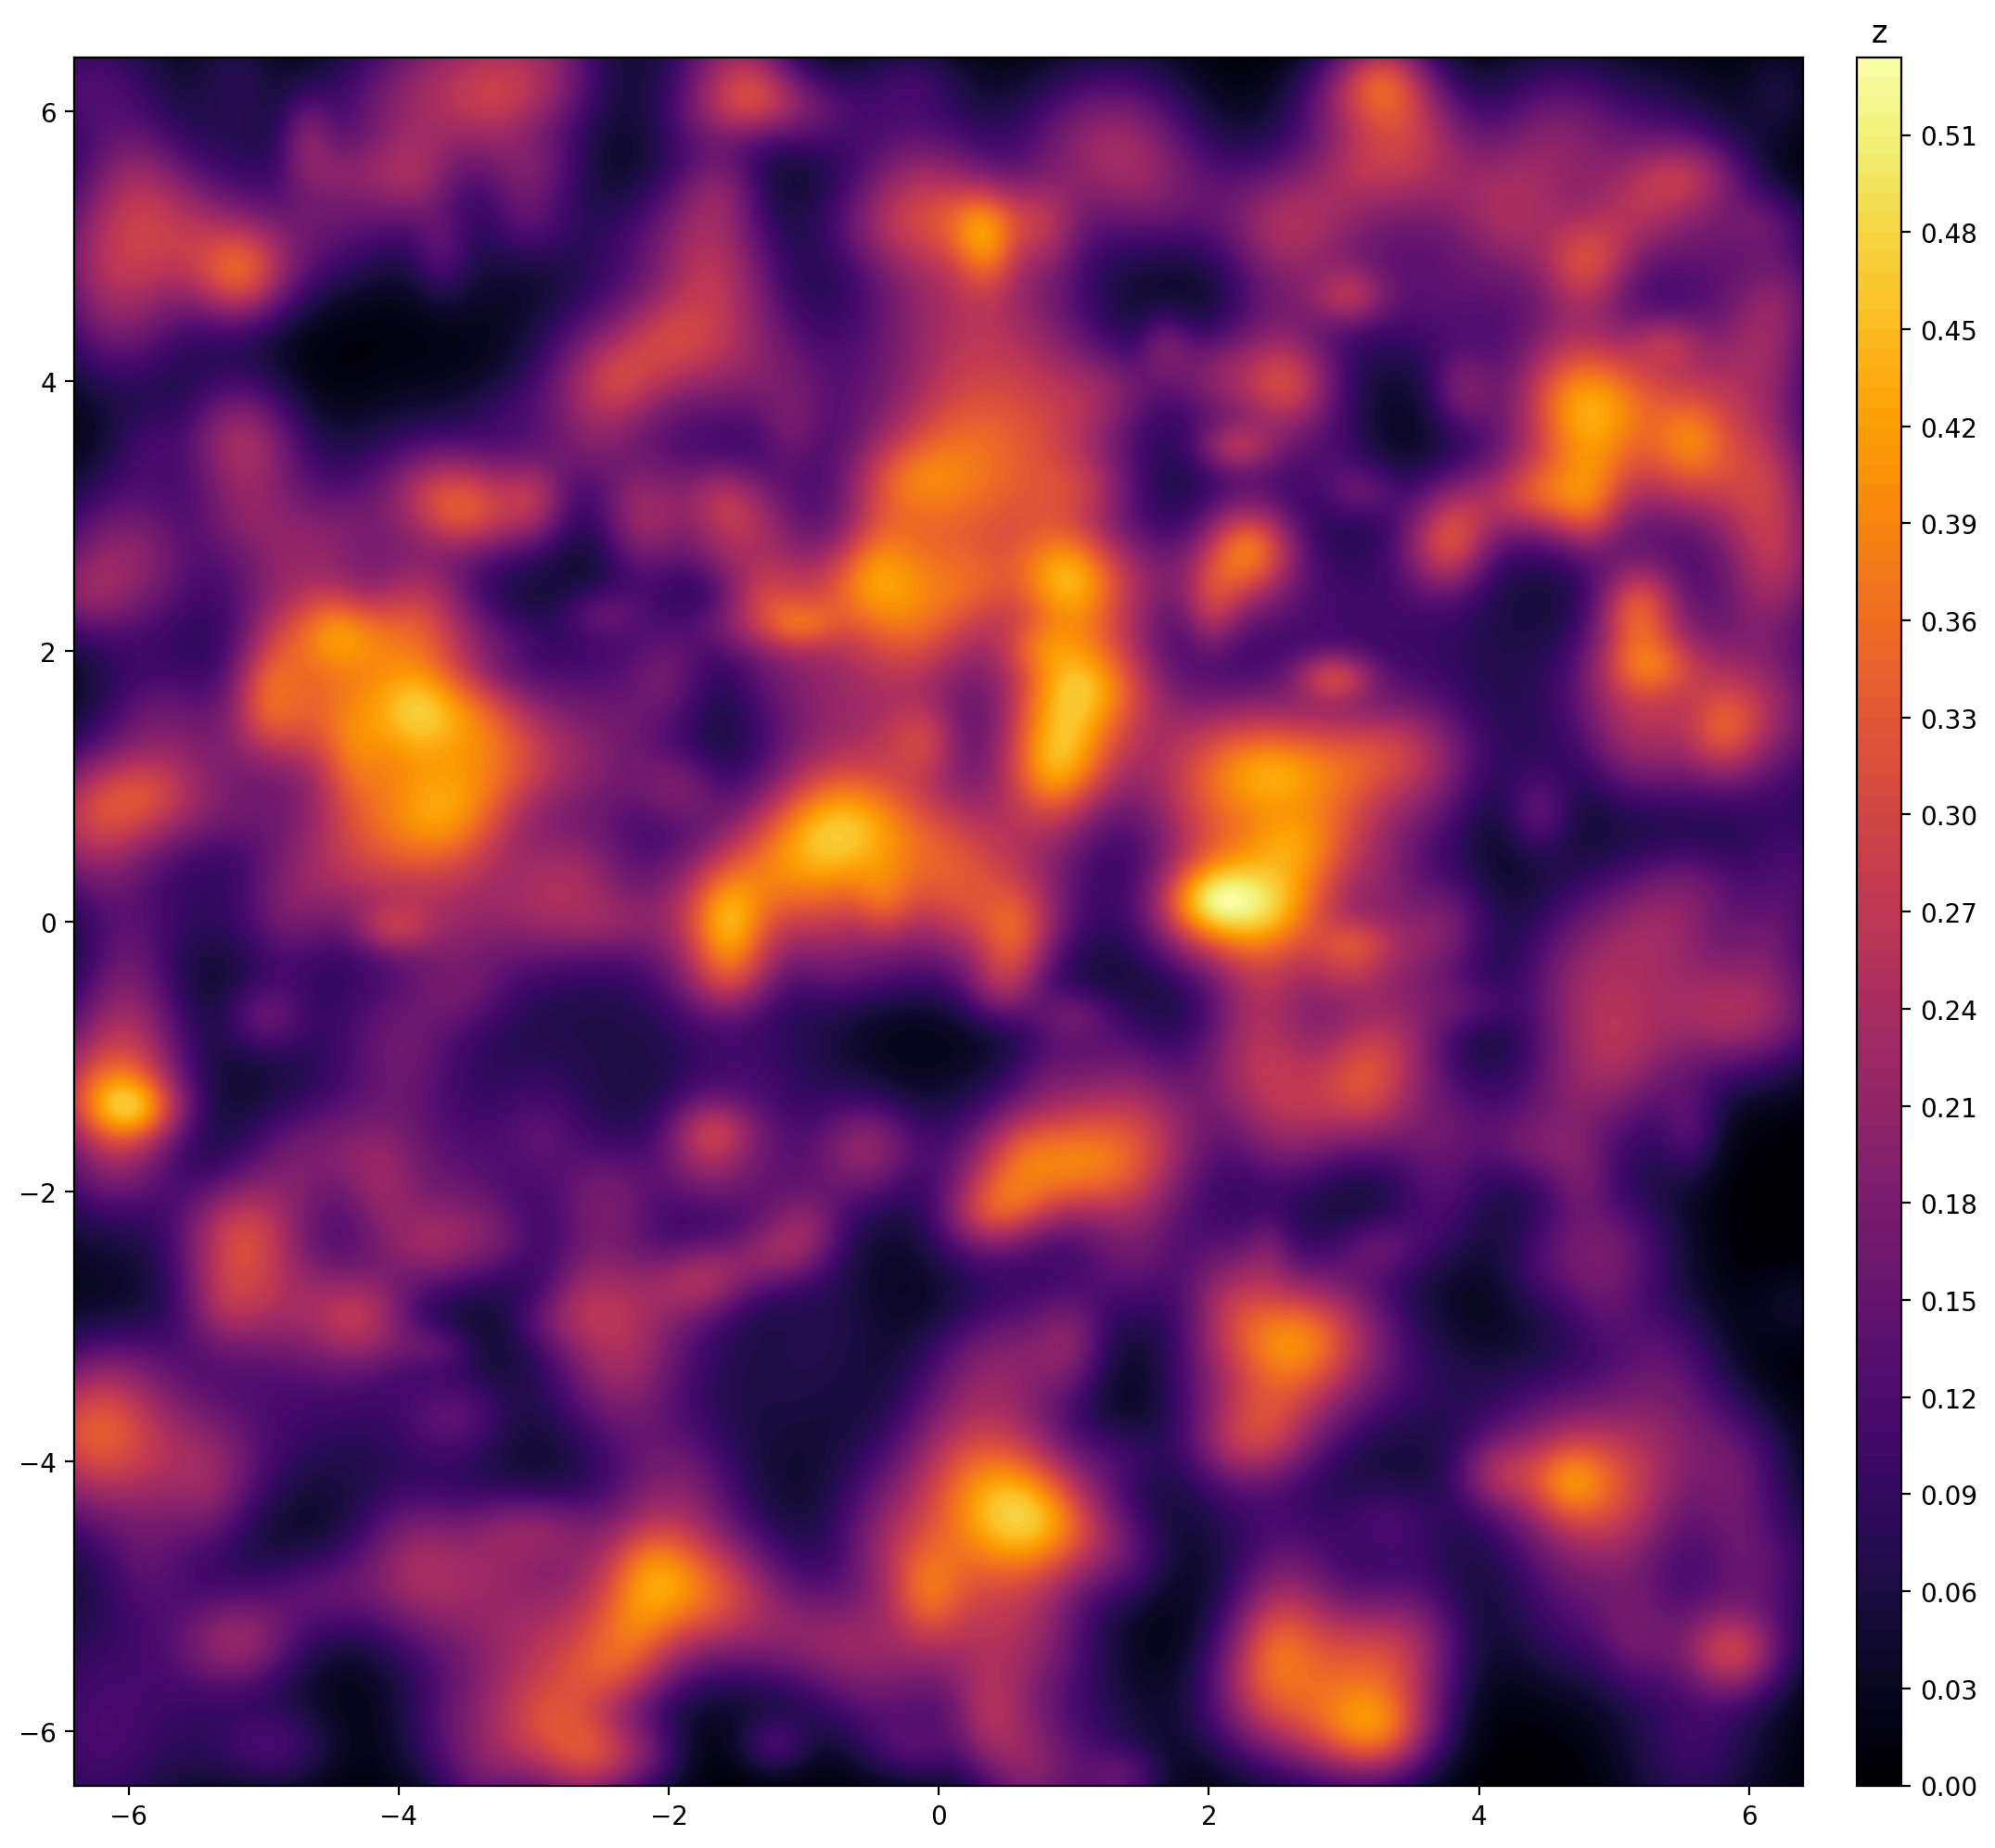
\includegraphics[width=0.5\textwidth]{fig/terrain_grid.png}
  \caption{Heightmap grid representing the terrain from Figure~\ref{fig:terrain}.}
  \label{fig:terrain_grid}
\end{figure}

\subsection{Robot-terrain interaction}
\label{sec:interaction}

To model the force interaction between the robot pointcloud and the terrain, we use a spring-damper system. If the robot were represented by a single point mass, the complete reaction force would be presented by just a single spring-damper. However, because we have a multi-point robot and compute the reaction forces pointwise, it is necessary to distribute the overall force magnitude across all of the interaction points. This can be achieved by normalizing by the total number of contact points. The force at continous world coordinates $(x,y,z)$ is computed as the reaction of the spring-damper system in the direction of the terrain normal at that point. 

Overall, we obtain a matrix of terrain reaction forces $\mathbf{F}_{\text{terrain}} = \left[\mathbf{f}_1 \, , \, \mathbf{f}_2 \, , \, \ldots \, , \, \mathbf{f}_N \right]$, where $\mathbf{f}_i$ is the force acting on the $i$-th point of the robot.
 given by Equation~\ref{eq:terrain_reaction}.

\begin{equation}
  \label{eq:terrain_reaction}
  \mathbf{f}_i = \llbracket z_i \leq 0\rrbracket \frac{\left[ -k \left(z_i - z_{\text{terrain}}\right) - b \left(\mathbf{v}_i \cdot \mathbf{n}_i\right) \right]}{C} \mathbf{n}_i
\end{equation}

where $k$ is the spring constant, $b$ is the damping constant, $z_i$ is the height of the $i$-th point, $z_{\text{terrain}}$ is the height of the terrain at the $i$-th point, $\mathbf{v}_i$ is the velocity of the $i$-th point, $\mathbf{n}_i$ is the terrain normal at coordinates $(x_i, y_i)$ ($\mathbf{p}_i = \left[ x_i , y_i , z_i\right]$). $C = \max (1, \sum_{i} \llbracket z_i \leq 0\rrbracket)$.
See \href{https://github.com/edavidk7/tracked_sim_rl/blob/d7b59702c6411e1dbda3be214524a2e22cceaac6/engine/engine.py#L55}{the implementation}.

\begin{figure}[H]
  \centering
  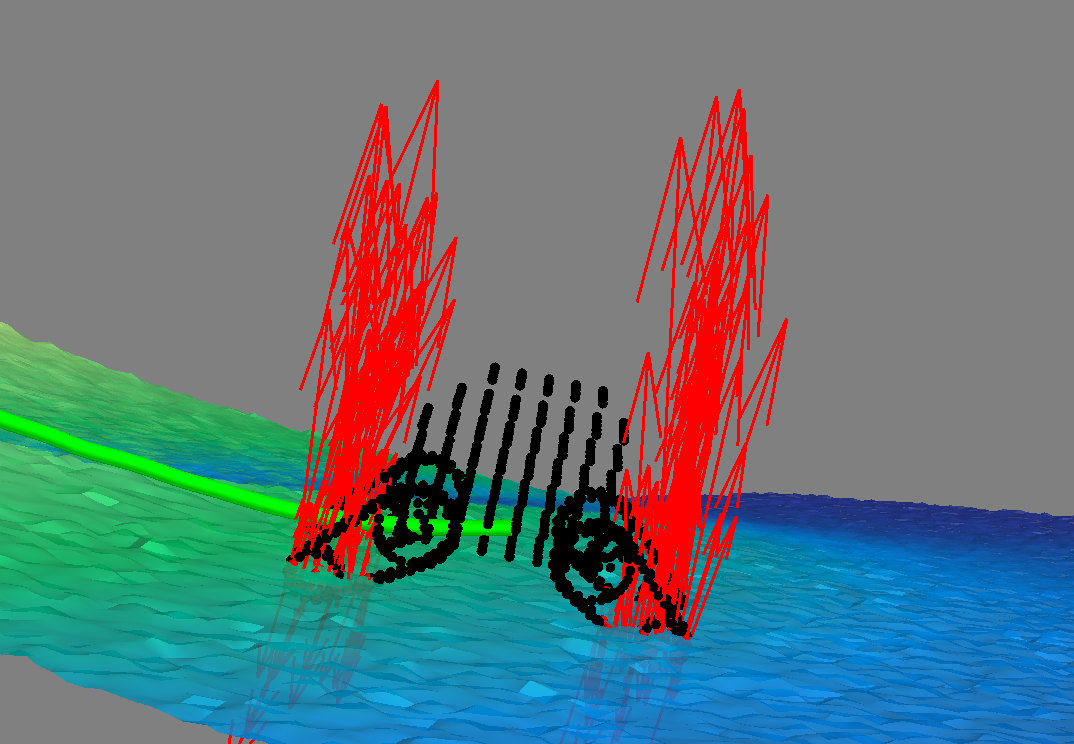
\includegraphics[width=0.8\textwidth]{fig/contact_forces.png}
  \caption{Terrain reaction force vectors during simulation.}
  \label{fig:terrain_reaction}
\end{figure}

\subsection{Friction and thrust calculation}
Having obtained the normal forces acting on each point of the robot in \ref{sec:interaction}, we can now compute the friction forces that generate the robot's thrust. We calculate the friction force's magnitude in a standard fashion as $\mu \left\| \mathbf{f}_i \right\|$, where $\mu$ is the friction coefficient. The direction of the friction force for a point is given by the difference between the commanded velocity of the robot's driving part and the current velocity of that point. We the project this difference onto the terrain's tanget plane at that point to obtain the friction force direction. The magnitude of the velocity difference is saturated using $\text{tanh}(\mathbf{x})$. The resulting friction force acting on the $i$-th point is given by Equation~\ref{eq:friction_force}.

\begin{equation}
  \label{eq:friction_force}
  \mathbf{f}_{\text{friction},i} = \mu \left\| \mathbf{f}_i \right\| \cdot \text{tanh}\left(  \Delta \mathbf{v}_i -  \left( \Delta \mathbf{v}_i\cdot \mathbf{n}_i \right) \mathbf{n}_i \right) 
\end{equation}

where $\Delta \mathbf{v}_i = \mathbf{v}_{i,\text{commanded}} - \mathbf{v}_i$. The use of tanh saturation means that whenever the difference in velocities grows large (e.g. robot is sliding down a slope), the friction force is saturated to a constant value. This is largely because when the robot is sliding perpendicularly to it's commanded velocity, the available friction is limited. This computation is implemented \href{https://github.com/edavidk7/tracked_sim_rl/blob/d7b59702c6411e1dbda3be214524a2e22cceaac6/engine/engine.py#L124}{here}.

\subsection{Simulating robot dynamics}
\label{sec:dynamics}

To simulate the robot's dynamics, we employ standard 6DoF rigid body model introduced by \citet{Agishev_2024}.

\begin{equation}
\label{eq:dynamics}
\begin{aligned}
    \dot{\mathbf{x}} &= \mathbf{v} \\
    \dot{\mathbf{v}} &= \frac{1}{M} \left( \mathbf{f}_g + \sum_i  \mathbf{f}_{i, \text{ext}}  \right)  \\
    \dot{\mathbf{R}} &= \boldsymbol{\omega} \times \mathbf{R} \\
    \dot{\boldsymbol{\omega}} &= \mathbf{I}^{-1} \sum_i \hat{\mathbf{p}}_i\times \mathbf{f}_{i, \text{ext}}
\end{aligned}
\end{equation}

where $\mathbf{x}$ is the robot's position, $\mathbf{v}$ is the robot's velocity, $\mathbf{R}$ is the robot's orientation, $\boldsymbol{\omega}$ is the robot's angular velocity, $M$ is the robot's mass, $\mathbf{I}$ is the robot's inertia tensor, $\mathbf{f}_{i, \text{ext}}$ is the external force acting on the $i$-th point, and $\hat{\mathbf{p}}_i$ is the vector from the robot's center of mass to the $i$-th point.

Implementation-wise, all variables are kept within the global world frame. This makes computation of the forces acting on the robot's points computationally less demanding because they are generated in the world frame,  see \href{https://github.com/edavidk7/tracked_sim_rl/blob/a6cfea8836db27df2154c90051075746729694d0/engine/engine.py#L48-L49}{code 1}, \href{https://github.com/edavidk7/tracked_sim_rl/blob/a6cfea8836db27df2154c90051075746729694d0/engine/engine.py#L65-L73}{code 2}.

A notable change, necessitated by the robot's changing geometry due to flipper articulation, is the computation of the robot's intertia tensor $\mathbf{I}$ and CoG. These have to be dynamically computed at each time step, as the robot's geometry changes, see \href{https://github.com/edavidk7/tracked_sim_rl/blob/a6cfea8836db27df2154c90051075746729694d0/engine/engine.py#L201}{code}.


\subsection{Simulation pipeline}
\label{sec:pipeline}

Putting all previously described steps together, we obtain the simulation pipeline. The pipeline is shown in Algorithm~\ref{alg:simulation_pipeline}.

\begin{algorithm}[H]
  \caption{Simulation Pipeline - see \href{tracked_sim_rl/blob/a6cfea8836db27df2154c90051075746729694d0/engine/engine.py}{code}}
  \label{alg:simulation_pipeline}
  \begin{algorithmic}
    \vspace{0.25cm}
    \STATE \textbf{Procedure} SimulateRobot(\textit{robot}, \textit{terrain}, \
    \textit{robot\_state}, \textit{control}, \textit{dt}, \textit{spring\_const}, \textit{damping\_const}, \textit{friction\_const})
        \STATE Compute terrain reaction forces $\mathbf{F}_{\text{terrain}}$ using Equation~\ref{eq:terrain_reaction}
        \STATE Compute friction forces $\mathbf{F}_{\text{friction}}$ using Equation~\ref{eq:friction_force}
        \STATE Compute robot dynamics using Equation~\ref{eq:dynamics}
        \RETURN Updated robot state
    \vspace{0.25cm}
    \end{algorithmic}

  \end{algorithm}

\clearpage
% RESULTS AND DISCUSSION
%------------------------------------------------------------------------
\section{Optimized implementation}
\label{sec:opt-impl}

\subsection{Computational complexity}

When viewed from a conventional standpoint, the simulation engine described above is still quite computationally demanding, especially for CPUs that perform mostly serial execution of instructions and have limited core counts. This is because of many matrix-vector and matrix-matrix multiplications, and sampling/interpolation from the terrain grid. When used with high-resolution robot geometry ($\sim$ 1000 points) and high-resolution terrain maps ($\sim$ 512x512), the simulation can become prohibitively slow, especially for larger number of simultanously simulated robots. Vector-matrix operations are in orders of $O(mn)$, where $m$, $n$ are the matrix dimensions. Matrix-matrix operations are in orders of $O(mnp)$. 

\subsection{GPU acceleration}

When viewed from the perspective of modern deep learning, the operations used in the simulation engine are ones widely used and supported when training deep neural networks. This means they are implemented in highly optimized libraries such as PyTorch \citep{paszke2019pytorchimperativestylehighperformance} with support for GPU acceleration, and modern GPUs contain hardware tailored for these operations. Furthermore, advanced algorithmic methods for optimizing sequences of such operations exist and are capable of generating highly optimized application-specific code. In our implementation we will leverage this and modify the standard code to optimize it for GPU execution.

\subsection{Conditions and branching}
A crucial step in optimizing the code for GPU is to avoid any sort of conditional branching. GPUs are designed for highly parallel execution of (identical) instructions, and any sort of deviation mid-execution leads to significant slowdowns, because the thread management has to stop and serialize execution on different branches. This doesn't impact only GPUs, even some superscalar modern CPUs benefit from conditionless code, assuming the problem size does not increase too much.

In the PyTorch-based implementation of the engine, special care had to be taken when implementing the masks of points that are in contact with the terrain and masks of points that belong to the robot's driving parts (tracks). Conventionally, one would use indexing with boolean masking such as \texttt{points[points[:,2] < 0]} to select points that are below the terrain. However, this would lead to a conditional branch, as well as a different shape of the resulting tensor in every iteration. All instances of such boolean masking were replaced by a very GPU-friendly operations of multiplication and addition. So, instead of \texttt{contact\_points = points[points[:,2] < 0]}, we use \texttt{contact\_points = points * (points[:,2] < 0).float()}, retaining the same shape and performing only an elementwise multiplication.

\subsection{Kernel compilation with PyTorch}
Since the release version 2.0, a new \texttt{compile} functionality is available in PyTorch. It allows for automatic tracing, optimization, and compilation of the code into a computational kernel which is able to perform the computation significantly faster by optimizations such as fusion of consecutive operations or avoiding repeated memory load/stores. On GPUs, it can also specifically split and benchmark different matrix multiplication algorithms based on the data's specific shape.

A slight downside is the necessity of fixed-shape data, however, after optimization performed in the previous section, this holds true for our simulation engine. With the torch compiler, we are able to achieve even more significant speedups than with the standard PyTorch operations.

\begin{figure}[H]
  \centering
  \includegraphics[width=0.6\textwidth]{fig/graph_diagram.pdf}
  \caption{Computation graph of the engine traced by PyTorch.}
  \label{fig:speedup}
\end{figure}

\clearpage

\section{Performance evaluation}

For the evaluation, we have used the MARV robot with 1000 points and a 256x256 terrain grid. The integration time step was set to 10 ms. We test the batch size in an exponential power-of-two fashion, starting from 1 robot up to 512 robots. 

First, we perform an evaluation on the CPU. In this case, it is an Apple M1 Pro chip with 10 cores and 16 GB of unified memory.

\begin{figure}[H]
  \centering
  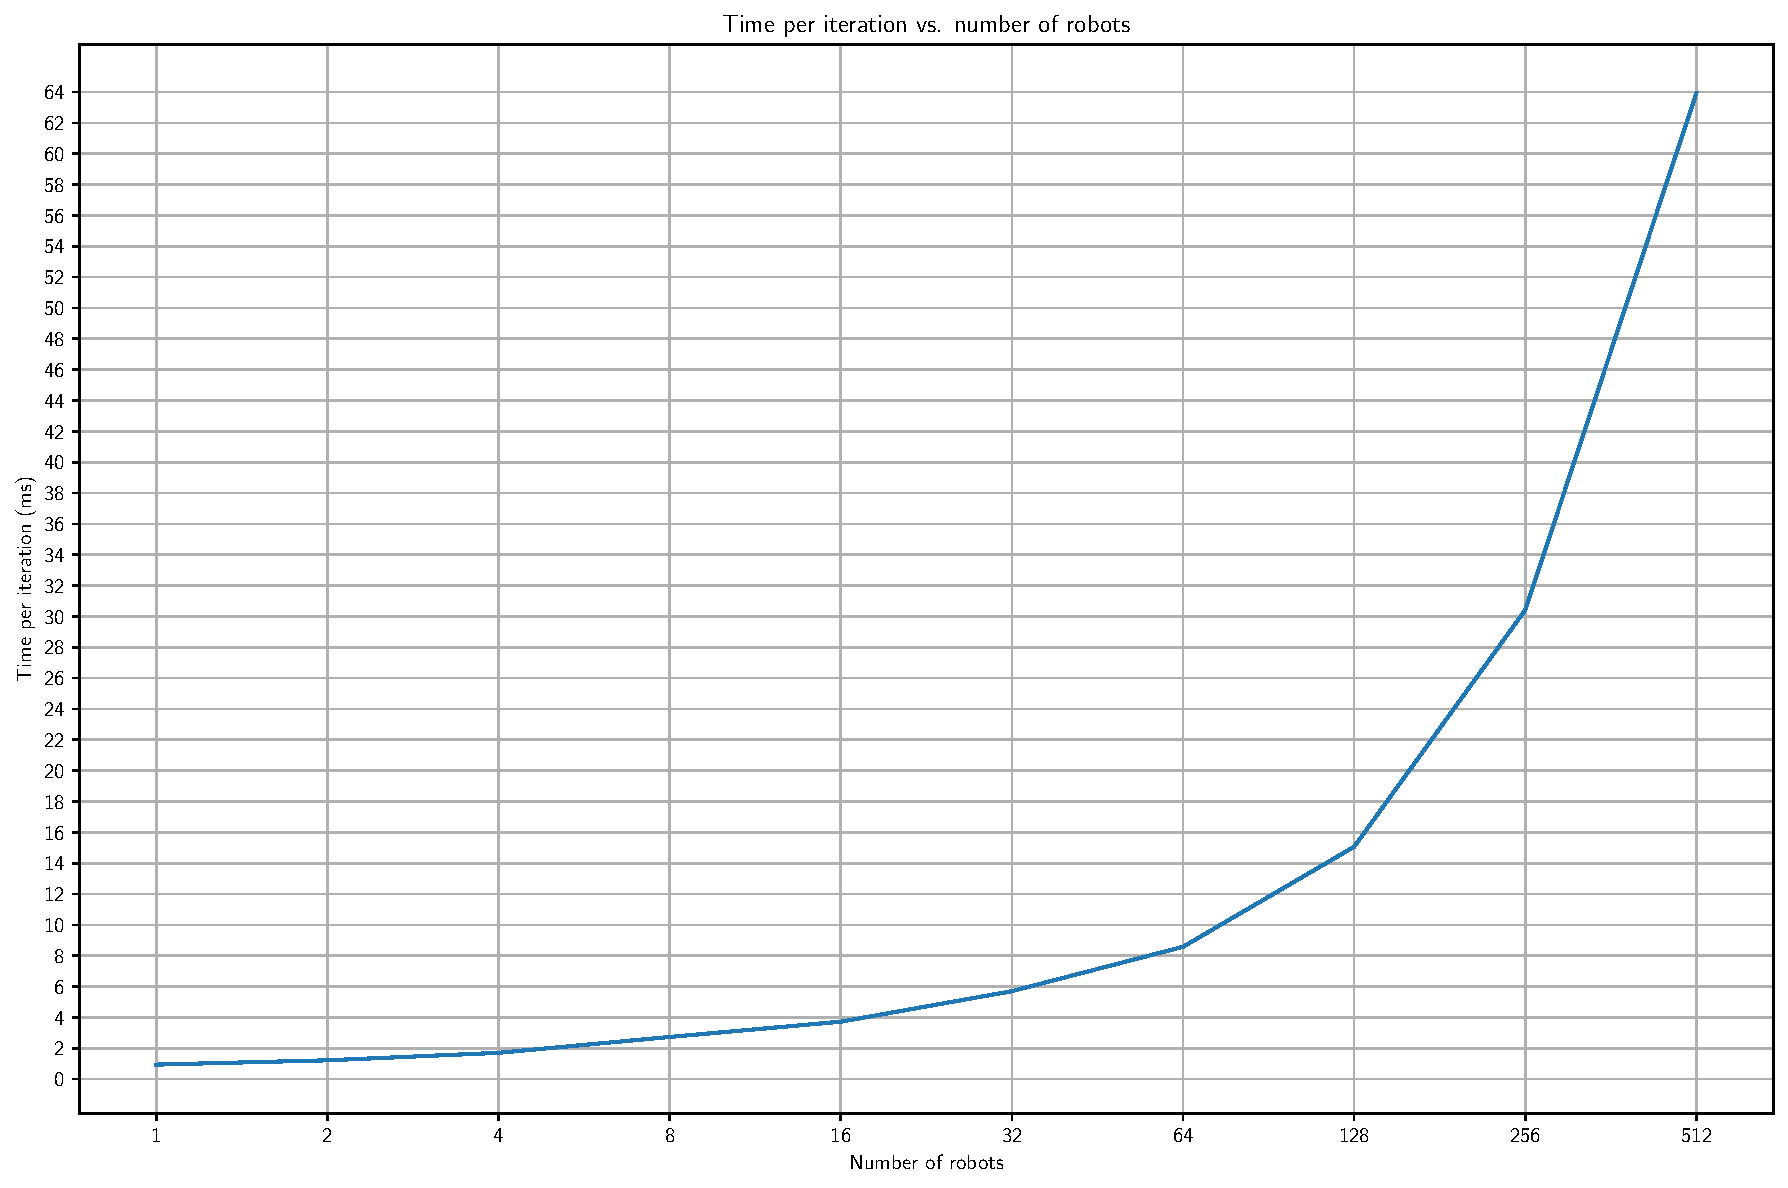
\includegraphics[width=1.\textwidth]{fig/benchmark_cpu_m1.pdf}
  \caption{Simulation speed with respect to the number of robots simulated - CPU. Note the logarithmic scale on the x-axis.}
  \label{fig:cpu_speedup}
\end{figure}

As expected, the simulation speed decreases with the number of robots. However, we notice slower increase in computation time for batch sizes of 8 or lower. This is possible due to the limited-size linear algebra units on the CPU, which have not yet been fully saturated. For the batch size of 128, a single iteration takes roughly 16 ms. This is slower than the real-time simulation, which is 10 ms. In comparison, however, a batch size of 1 takes around 1 ms. This gives us a (128 * 1 ms) / 16 ms = 8x speedup by batched parallelization instead of simulating robots one by one. If we were to compute the total robot simulation time compared to realtime driving, we get (128 * 10 ms) / 16 ms = 80x speedup.

\clearpage


Second, we perform the same evaluation on the GPU. In this case, it is an Nvidia A100 SXM4 with 40 GB of VRAM.

\begin{figure}[H]
  \centering
  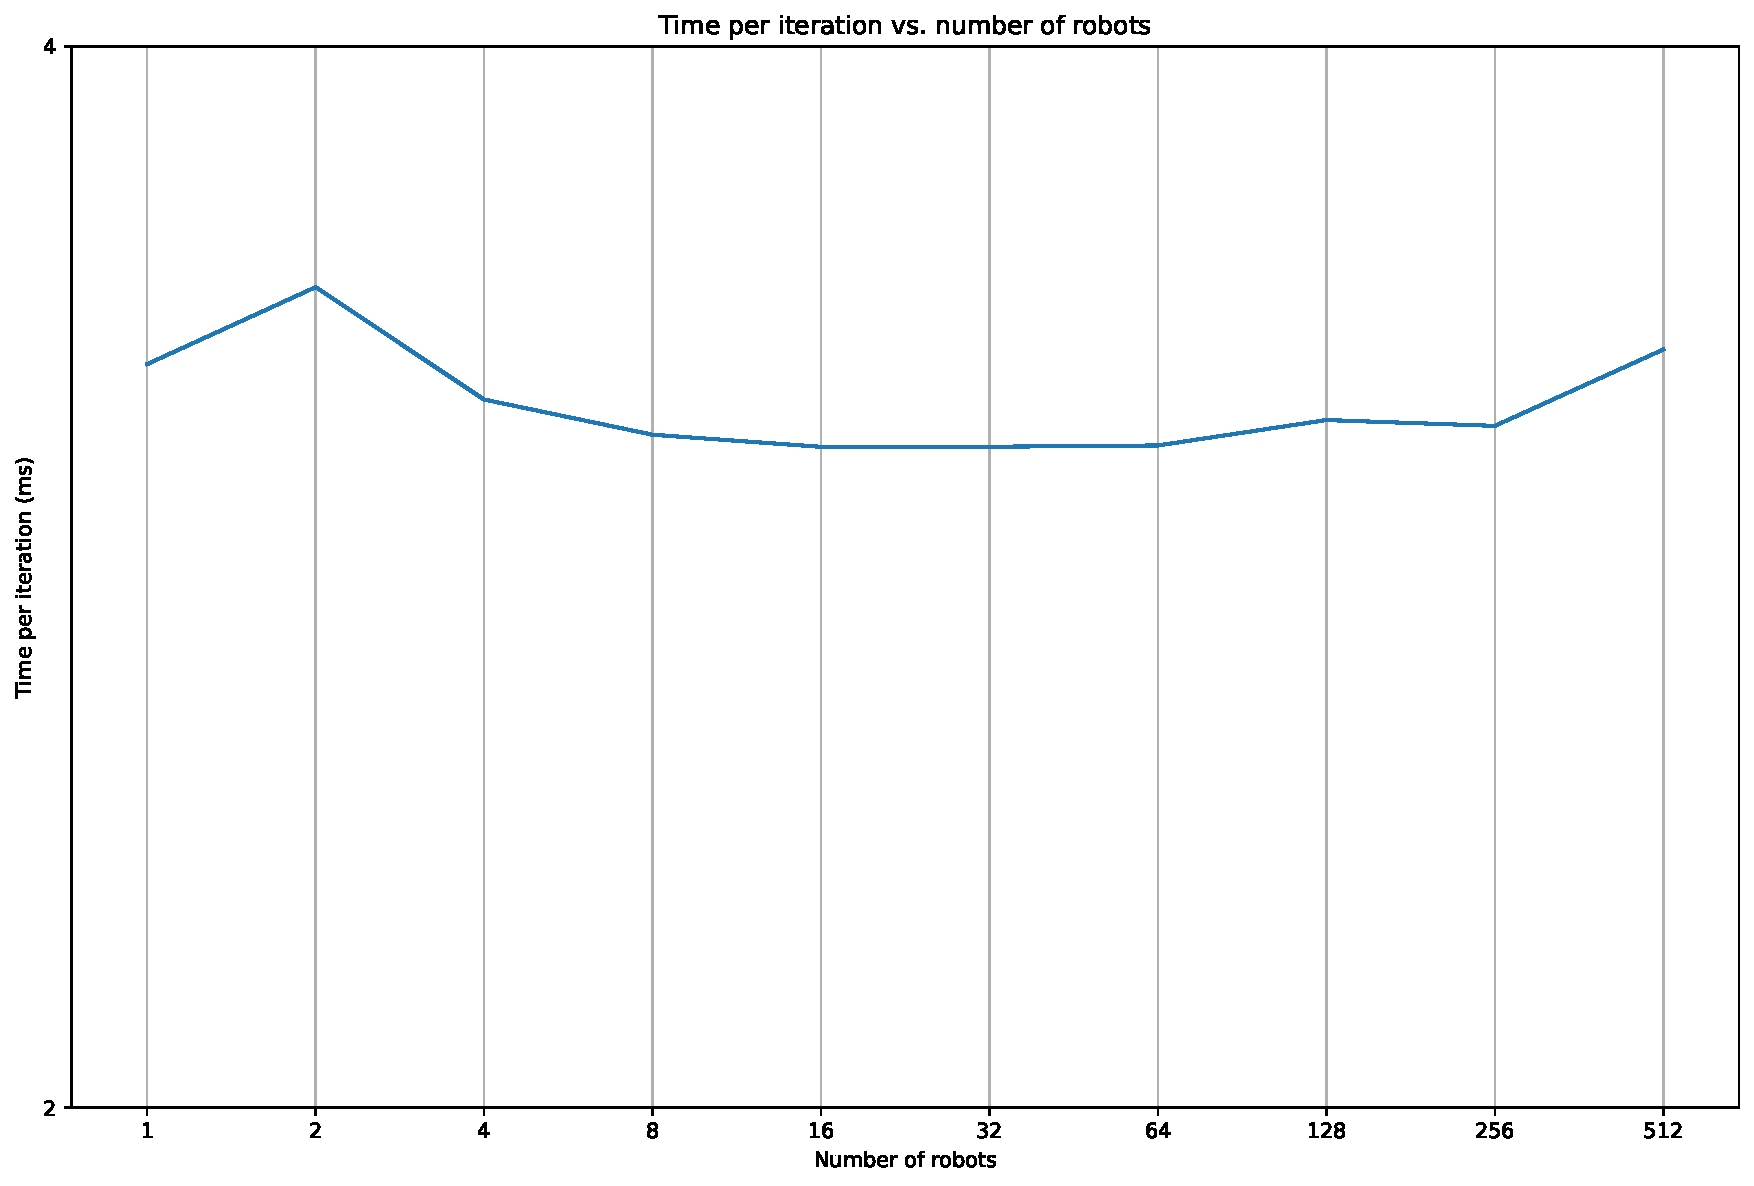
\includegraphics[width=1.\textwidth]{fig/benchmark_cuda_2025-01-12_21-41-37_eager.pdf}
  \caption{Simulation speed with respect to the number of robots simulated - GPU. Note the logarithmic scale on the x-axis.}
  \label{fig:gpu_speedup}
\end{figure}

It is notable that the GPU slightly slower for batch sizes smaller than 8, likely due to synchronization and data overhead. However, the speedup is much more significant than on the CPU. Increasing the batch size up to 512 does not change the computation time significantly. The simulation time is constantly about 3.5 ms. This gives us a (512 * 10 ms) / 3.5 ms = 1462x speedup compared to real-time driving. Or about 10 ms / 3.5 ms = 2.8x speedup over realtime.

As expected, the GPU is significantly faster than the CPU, especially for larger batch sizes.

\clearpage
\section{Reinforcement learning environment}

As a part of the project, we have developed a generic reinforcement learning environment based on the TorchRL library \citep{bou2023torchrldatadrivendecisionmakinglibrary}. TorchRL provides native interop with PyTorch's Tensor datatype as well as the use of various accelerators (torch "devices"). As our pipeline was designed to operate completely on the GPU, this improves efficiency by avoiding data transfers between GPU VRAM and system RAM. Libraries such as the Gymnasium \citep{towers2024gymnasiumstandardinterfacereinforcement} are meant to run and output numpy arrays, forcing the use of a CPU. TorchRL comes preimplemented with a number of deep reinforcement learning algorithms and offers a relatively lightweight interface for defining custom environments.

\subsection{Observations and actions}
To simulate possible perception inputs for the robot, we implemented two basic sensor types. The first is a bird-view "camera", which provides a 2D image of the robot's surroundings. The image is centered on top of the robot and provides a 360-view of the surrounding environment. The values of the pixels are,however, not RGB values but rather the metric height of the terrain at that point. 

The second sensor is a 3D LiDAR, which provides a 360 degree pointcloud of the robot's surroundings. It is in essence similar to the camera, except the data are not structured in a grid and contain the x,y,z coordinates of the points in robot's local frame.

\begin{figure}[H]
  \centering
  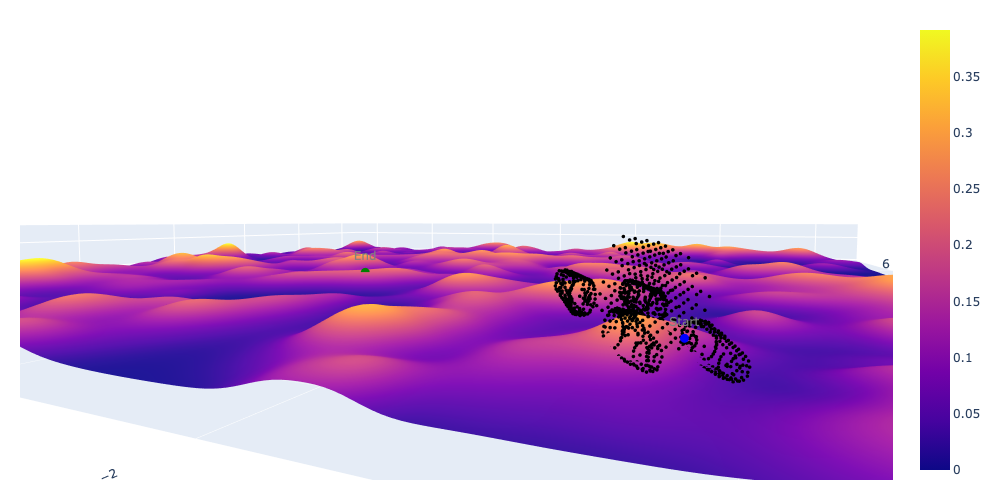
\includegraphics[width=0.9\textwidth]{fig/robot_on_terrain.png}
  \caption{Robot during an environment rollout.}
\end{figure}

\begin{figure}[H]
  \centering
  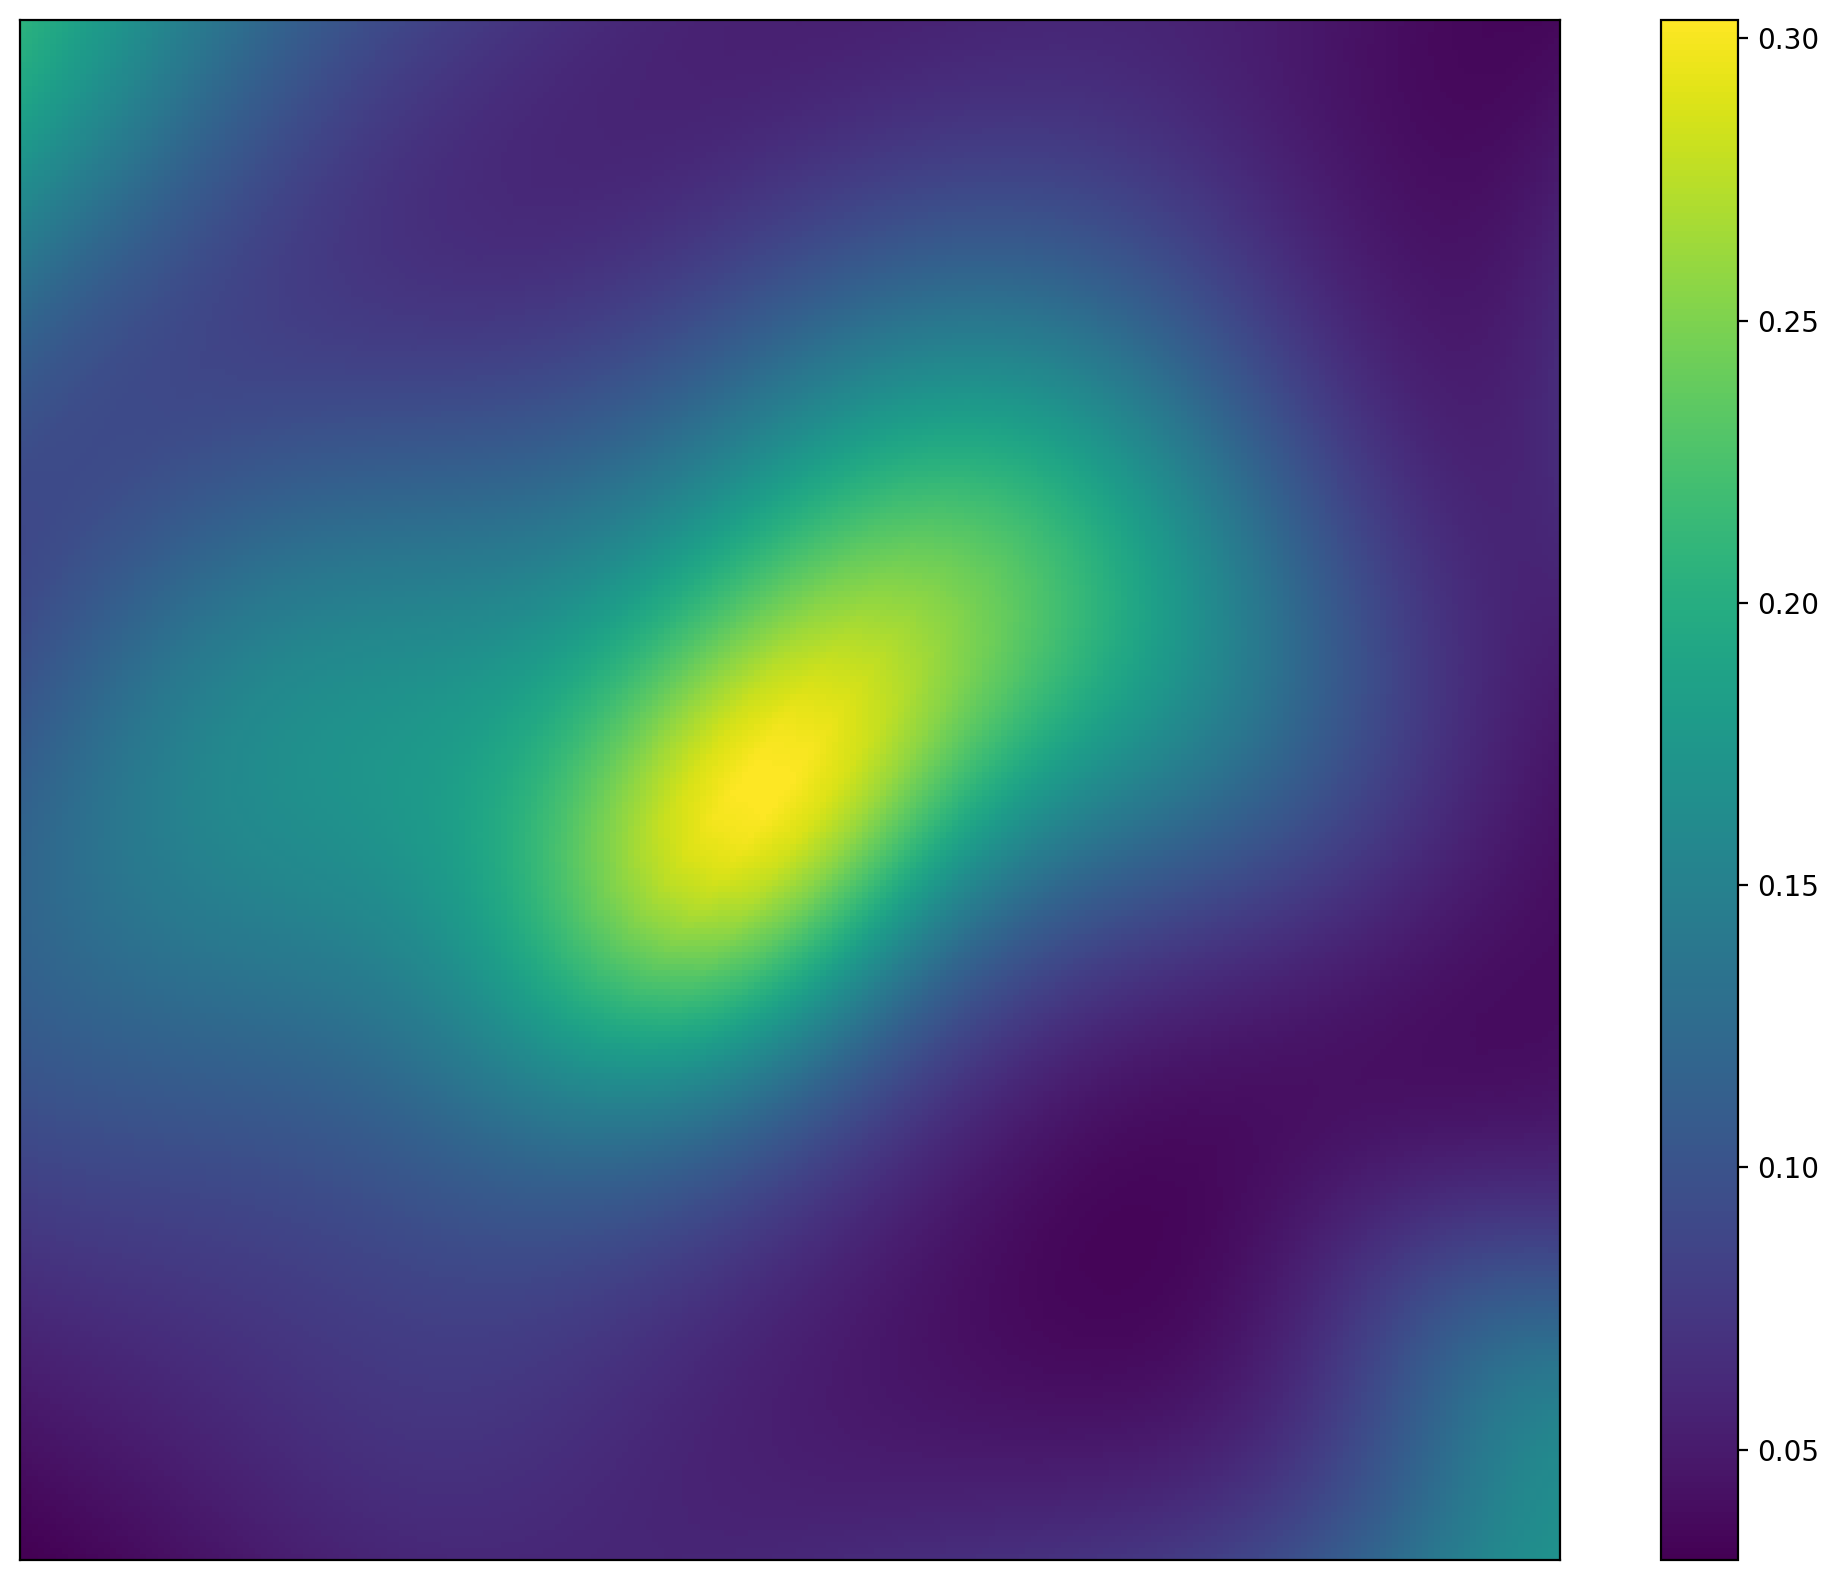
\includegraphics[width=0.6\textwidth]{fig/birdview_camera.png}
  \caption{Bird-view camera sensor output.}
\end{figure}
\begin{figure}[H]
  \centering
  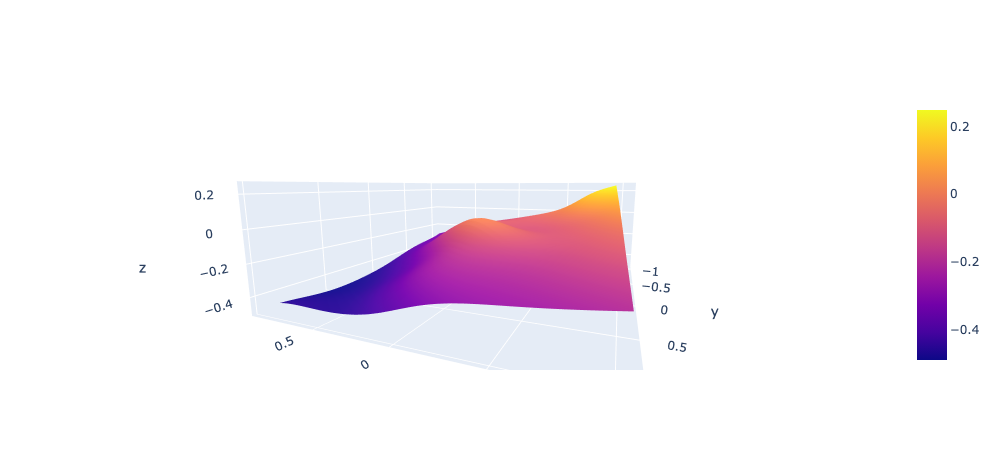
\includegraphics[width=0.9\textwidth]{fig/pointcloud.png}
  \caption{LiDAR sensor output.}
\end{figure}

\clearpage
\subsection{Terrain generation}
To allow for training in diverse, unseen environments, we implemented a simple terrain generator. The generator is based on addition of randomly generated gaussian functions. The generator is parameterized in way that allows for both smooth and rough terrains controlled by interpretable parameters. See the \href{https://github.com/edavidk7/tracked_sim_rl/blob/d7b59702c6411e1dbda3be214524a2e22cceaac6/utils/heightmap_generators.py#L71}{code}.

\begin{figure}[H]
  \centering
  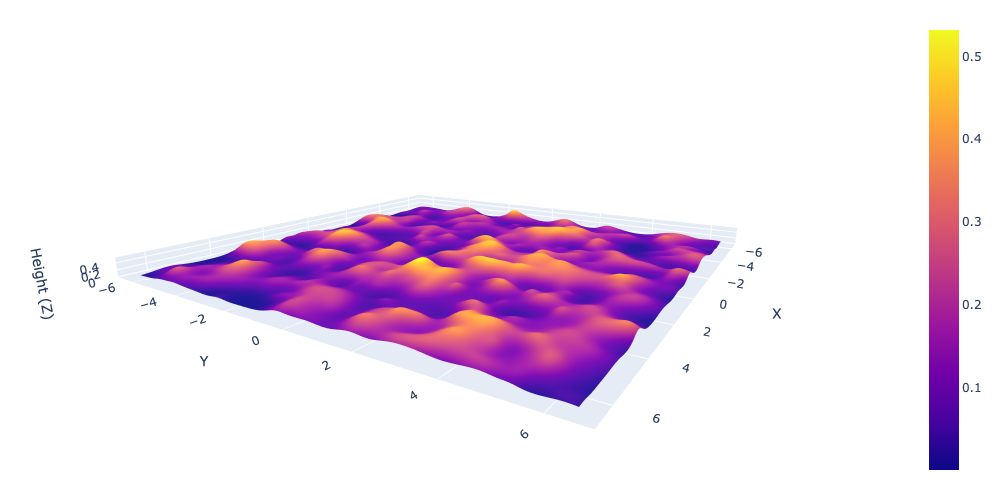
\includegraphics[width=0.9\textwidth]{fig/rough_terrain.png}
  \caption{Generated terrain with rough preset.}
\end{figure}

\begin{figure}[H]
  \centering
  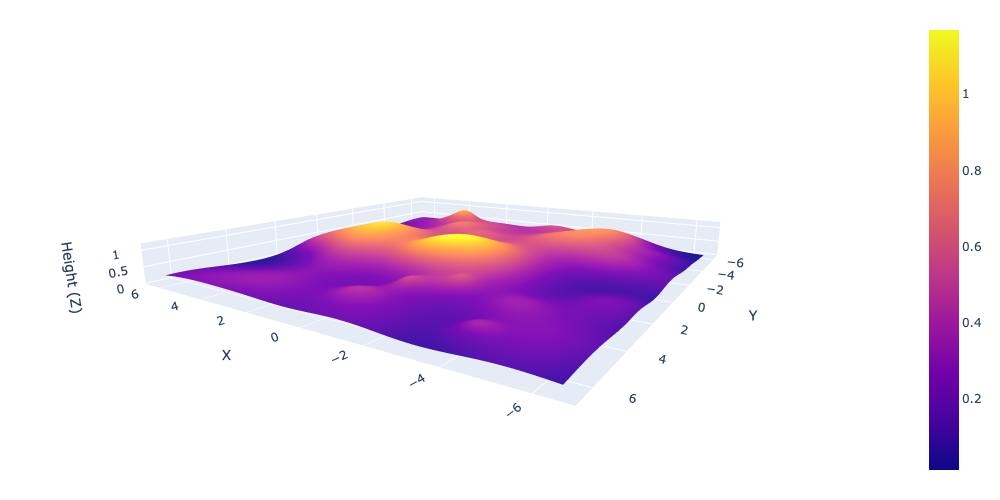
\includegraphics[width=0.9\textwidth]{fig/smooth_terrain.png}
  \caption{Generated terrain with smooth preset.}
\end{figure}
% CONCLUSIONS
%------------------------------------------------------------------------
\section{Conclusion}
\label{sec:conclusion}

We developed and implemented a high-performance, GPU-compatible simulation engine for tracked robots used by the Vision for Robotics and Autonomous Systems group. The engine is capable of simulating multiple robots at once, and is optimized for GPU execution. We have also developed a reinforcement learning environment based on the TorchRL library with two types of sensors, a bird-view camera and a 3D LiDAR, and a terrain generator capable of generating diverse terrains.

Unfortunately, due to initial problems with the implementation of the engine by \citet{Agishev_2024}, we were unable to complete RL training on the robots. However, the engine is fully functional and ready for use in future projects.

\clearpage

% REFERENCES
%------------------------------------------------------------------------
\bibliographystyle{report_template}
\bibliography{references}
\addcontentsline{toc}{section}{References} %Add this to the contents page


\end{document}



